
%_________Mainpart__________________________________

\chapter{System Identification}
\label{chap:system_identification}

The target of the system identification is to estimate the kinematics of the object, which are:
\begin{enumerate}
	\item mass $m$
	\item center of gravity, represented through the offset $\vec c$ from the grasping point to the center of gravity
	\item inertia matrix $\vec I_\scr{q}$, with respect to the center of gravity
\end{enumerate}

For simplicity we will first discuss the problem of the identification of the object kinematics with only one grasping point. Starting from these formulas, we will then continue with multiple grasping points, which is the case for cooperative identification.

\section{One Grasping Point}
\label{sec:one_grasping_point}

\begin{figure}
	\centering
	\begin{tikzpicture}
	% world frame
	\draw[arrows=->,line width=0.4pt] (0, 0) -- (0.5, 0);
	\draw[arrows=->,line width=0.4pt] (0, 0) -- (0.35, 0.35);
	\draw[arrows=->,line width=0.4pt] (0, 0) -- (0, 0.5);
	\node at (0.8, 0) {$^wx$};
	\node at (0.5, 0.5) {$^wy$};
	\node at (0, 0.8) {$^wz$};
	\node at (-0.1, -0.3) {$W$};
	
	% load
	\draw[fill,light-gray,draw=black] plot[smooth, tension=1.3] coordinates {(2, 2) (3, 4) (6, 3) (4, 2) (5, 0.5) (3, 0.2) (2, 2)};
	
	% load frame
	\draw[arrows=->,line width=0.4pt] (3, 3.8) -- (3.35, 3.45);
	\draw[arrows=->,line width=0.4pt] (3, 3.8) -- (2.45, 3.65);
	\draw[arrows=->,line width=0.4pt] (3, 3.8) -- (3.1, 4.2);
	\node at (3.55, 3.25) {$^lx$};
	\node at (2.25, 3.65) {$^ly$};
	\node at (3.1, 4.4) {$^lz$};
	\node at (3, 3.5) {$L$};
	
	% gripper
	\draw[draw=black,line width=2pt] (3.1, 4) -- (3.45, 3.65);
	\draw[draw=black,line width=2pt] (2.7, 3.9) -- (3.05, 3.55);
	\draw[draw=black,line width=2pt] (3.1, 4) -- (2.7, 3.9);
	\draw[draw=black,line width=2pt] (2.6, 4.3) -- (2.95, 3.95);
\end{tikzpicture} 
	\caption{Load with one grasping point}
	\label{fig:load_one_grasping_point}
\end{figure}

The system behaviour of a model like \ref{fig:load_one_grasping_point} can be described through 
\begin{equation}
	^\scr{L}\vec{F} = m {^\scr{W}}\vec{\ddot{p}} + m ^\scr{L}\vec{g} + ^\scr{L}\vec{\dot{\omega}} \times m ^\scr{L}\vec{c} + ^\scr{L}\vec{\omega} \times (^\scr{L}\vec{\omega} \times m ^\scr{L}\vec{c}),
	\label{eq:force}
\end{equation}
which is derived from the conservation of momentum, and
\begin{equation}
	^\scr{L}\vec{N} = ^\scr{L}\vec{I}_\scr{p} ^\scr{L}\vec{\dot{\omega}} + ^\scr{L}\vec{\omega} \times (^\scr{L}\vec{I}_\scr{p} ^\scr{L}\vec{\omega}) + m ^\scr{L}\vec{c} \times {^\scr{W}}\vec{\ddot{p}} + m ^\scr{L}\vec{c} \times ^\scr{L}\vec{g},
	\label{eq:torque}
\end{equation}
which comes from the conservation of angular momentum. Both formulas are taken from \cite{literaturstelle1}, but are used here with a different definition of the gravity vector. Throughout this paper we assume that in the world coordinate frame $\vec g$ only has a component in the $z$-direction, with a negative value.

The inertia matrix $\vec I_\scr{p}$ in these formulas represents the inertia of the object transformed into the grasping point through the parallel axis theorem
\begin{equation}
	\vec I_\scr{p} = \vec I_\scr{q} + m \left( (\vec c^\scr{T} \vec c) \vec 1 - (\vec c \vec c^\scr{T}) \right).
\end{equation}
All values, besides the position of the object $\vec p$, are represented in the load frame, as for instance the angular velocity $\vec \omega$ of the endeffector. This value can be calculated as the derivative with respect to time of the orientation $^W\vec{\varphi}$ of the load coordinate frame in the world coordinate frame:
\begin{equation}
	{^\scr{W}}\vec{\omega} = \frac{\partial {^\scr{W}}\vec{\varphi}}{\partial t}
\end{equation}
For use in the estimator this value needs to be transformed into the load coordinate frame, which means that the rotation
\begin{equation}
	^\scr{L}\vec{\omega} = \vec{R}({^\scr{W}}\vec{\varphi}) {^\scr{W}}\vec{\omega}
\end{equation}
must be applied. For the graviation, which changes its direction in the load coordinate frame with the rotation of the object, the same rotation is necessary. For the sake of legibility we will not denote the coordinate frames anymore during the rest of this section.

In the case of only one grasping point we then have in total ten unknowns:
\begin{enumerate}
	\item mass $m$
	\item grasping point offset from the center of gravity $\vec c = [c_x, c_y, c_z]^\scr{T}$ with three unknowns
	\item inertia matrix with six unknowns, as this matrix is by definition symmetric
	\begin{equation}
		\vec{I}_\scr{p} = 
		\begin{bmatrix}	
			I_{xx}	& I_{xy}	& I_{xz} \\
			I_{xy}	& I_{yy}	& I_{yz} \\
			I_{xz}	& I_{yz}	& I_{zz}
		\end{bmatrix}
	\end{equation}
\end{enumerate}

These values are combined to the system parameter vector
\begin{equation}
	\vec{\Theta} = [m, m c_x, m c_y, m c_z, I_{xx}, I_{xy}, I_{xz}, I_{yy},I_{yz}, I_{zz}]^\scr{T},
\end{equation}
where in practice we do not know the correct values, but instead only the estimation $\vec{\hat \Theta}$.

For the estimator as input information we have a vector filled with the forces and torques at the grasping point
\begin{equation}
	\vec{h} = [F_x, F_y, F_z, M_x, M_y, M_z]^\scr{T},
\end{equation}
the position of the grasping point $\vec p$, the angular velocity $\vec \omega$ of the grasping point and the gravity $\vec g$. For a recursive least squares estimation we need now the linear relation
\begin{equation}
	\vec{h}(k) = \vec{\Phi}(k) \vec{\Theta}(k)
\end{equation}
between $\vec{\Theta}$ and $\vec{h}$ with
\begin{equation}
	\vec{\Phi}(k) = 
	\begin{bmatrix}
		\vec{\ddot p} - \vec{g}	& [\vec{\dot \omega} \times] + [\vec{\omega}\times] [\vec{\omega} \times]	& 0 \\
		0			& [(\vec{g} - \vec{\ddot p}) \times]									& [.  \vec{\dot \omega}] + [\vec{\omega} \times] [. \vec{\omega}]
	\end{bmatrix},
\end{equation}
which was derived in \ref{MISSING}.

The recursive least squares is then an iterative improvement of the estimation, where for every sampling step the formulas
\begin{equation}
	\vec{K}(k) = \vec{P}(k-1) \vec{\Phi}^\scr{T}(k) (\vec{I} + \vec{\Phi}(k) \vec{P}(k - 1) \vec{\Phi}^\scr{T}(k))^{-1}
\end{equation}
\begin{equation}
	\vec{P}(k) = (\vec{I} - \vec{K}(k) \vec{\Phi}(k)) \vec{P}(k - 1)
\end{equation}
\begin{equation}
	\vec{\hat \Theta}(k)=\vec{ \hat \Theta}(k - 1) + \vec{K}(k) (\vec{h}(k) - \vec{\Phi}(k) \vec{\hat \Theta}(k - 1))
\end{equation}
are applied \ref{MISSING}. The initialization of the algorithm can be done through
\begin{equation}
	\vec{P}(k_0) = \left( \vec{\Phi}^\scr{T}(k_0) \vec{\Phi}(k_0) \right)^{-1}
\end{equation}
and
\begin{equation}
	\vec{\hat \Theta} (k_0) = \vec{P}(k_0) \vec{\Phi}^\scr{T}(k_0) \vec{h}(k_0).
\end{equation}

\section{Multiple Grasping Points}
\label{sec:multiple_grasping_points}
\begin{figure}
	\centering
	\resizebox{4cm}{!}{
\begin{tikzpicture}
	% world frame
	\draw[arrows=->,line width=0.8pt] (0, 0) -- (0.5, 0);
	\draw[arrows=->,line width=0.8pt] (0, 0) -- (0.35, 0.35);
	\draw[arrows=->,line width=0.8pt] (0, 0) -- (0, 0.5);
	\node at (0.8, 0) {{$^\mathrm{W}x$}};
	\node at (0.5, 0.5) {{$^\mathrm{W}y$}};
	\node at (-0.1, 0.8) {{$^\mathrm{W}z$}};
	\node at (-0.1, -0.3) {W};	
	% load
	\draw[fill,light-gray,draw=black] plot[smooth, tension=1.3] coordinates {(2, 2) (3, 4) (6, 3) (4, 2) (5, 0.5) (3, 0.2) (2, 2)};
	
	% load frame
	\draw[draw=blue,arrows=->,line width=0.8pt] (3, 3.8) -- (3.35, 3.45);
	\draw[draw=blue,arrows=->,line width=0.8pt] (3, 3.8) -- (2.45, 3.65);
	\draw[draw=blue,arrows=->,line width=0.8pt] (3, 3.8) -- (3.1, 4.2);
	\node[text=blue] at (3.55, 3.25) {{$^\mathrm{L}x$}};
	\node[text=blue] at (2.25, 3.9) {{$^\mathrm{L}y$}};
	\node[text=blue] at (3.1, 4.4) {{$^\mathrm{L}z$}};
	
		
	
	
	% gripper one
	\draw[draw=black,line width=2pt] (3.1, 4) -- (3.45, 3.65);
	\draw[draw=black,line width=2pt] (2.7, 3.9) -- (3.05, 3.55);
	\draw[draw=black,line width=2pt] (3.1, 4) -- (2.7, 3.9);
	\draw[draw=black,line width=2pt] (2.6, 4.3) -- (2.95, 3.95);
	\node at (2.6, 4.6) {$1$};
	
	% gripper two
	\draw[draw=black,line width=2pt] (2.8, 0.5) -- (3.1, 0.3);
	\draw[draw=black,line width=2pt] (2.8, 0.5) -- (3.1, 0.8);
	\draw[draw=black,line width=2pt] (3.1, 0.3) -- (3.4, 0.6);
	\draw[draw=black,line width=2pt] (2.65, 0.1) -- (2.95, 0.4);
	\node at (2.4, 0.2) {$2$};
	
	% gripper three
	\draw[draw=black,line width=2pt] (5.1, 2.9) -- (5.45, 2.55);
	\draw[draw=black,line width=2pt] (4.7, 2.8) -- (5.05, 2.45);
	\draw[draw=black,line width=2pt] (5.45, 2.55) -- (5.05, 2.45);
	\draw[draw=black,line width=2pt] (5.65, 2.15) -- (5.3, 2.5);
	\node at (5.9, 2.2) {$3$};
	
	% grasping offsets
	\draw[arrows=->,line width=1pt] (3, 3.8) -- (3.15, 0.55);
	\node at (3.6, 0.9) {$^\scr{L}\vec{r}_{12}$};
	\draw[arrows=->,line width=1pt] (3, 3.8) -- (5.1, 2.7);
	\node at (5.1, 3.2) {$^\scr{L}\vec{r}_{13}$};
	
	\draw[->,thick,dashed,green](0, 0) -- (3, 3.8);
	\node[text=blue] at (2.7, 3.3) {L};
	\node[text=green] at (0.8, 1.7) {$^\scr{W}\vec{p}$};
\end{tikzpicture}
}
	\caption{Load with multiple grasping points}
	\label{fig:load_multiple_grasping_points}
\end{figure}

Of course a load can also be hold by multiple manipulators, or arms in case of a human. As long as on every grasping point a force and torque sensor is mounted the basic principle of the previous section can be reused for the load estimation. In this case the forces and torques are distributed over all grippers, whereas the distribution depends on the reactive forces of the manipulators. Therefore, the only difference in the physics is that $n$ forces and torques are combined on the left hand sides of
\begin{equation}
	\sum_{i = 1}^{n}  {^\scr{L}}\vec{F}_{i} = m {^\scr{W}}\vec{\ddot{p}} + m {^\scr{L}}\vec{g} + {^\scr{L}}\vec{\dot{\omega}} \times m {^\scr{L}}\vec{c} + {^\scr{L}}\vec{\omega} \times ({^\scr{L}}\vec{\omega} \times m {^\scr{L}}\vec{c})
	\label{eq:force_multiple}	
\end{equation}
and
\begin{equation}
	\sum_{i = 1}^n {^\scr{L}}\vec{N}_{i} + \sum_{i = 2}^n {^\scr{L}}\vec{r}_{1i} \times {^\scr{L}}\vec{F}_{i} = {^\scr{L}}\vec{I}_\scr{p} {^\scr{L}}\vec{\dot{\omega}} + {^\scr{L}}\vec{\omega} \times ({^\scr{L}}\vec{I}_\scr{p} {^\scr{L}}\vec{\omega}) + m {^\scr{L}}\vec{c} \times {^\scr{W}}\vec{\ddot{p}} + m {^\scr{L}}\vec{c} \times {^\scr{L}}\vec{g}.
	\label{eq:torque_multiple}	
\end{equation}
The additional summands for the torques are caused by the forces which are not applied in the grasping point one. Implicitly for these formulas we assume that the load coordinate system has its origin in the grasping point of gripper one and that the offsets ${^\scr{L}}\vec{r}_{1i}$ from this gripper to the gripper $i$ are known. Additonally, we have again denoted the corresping coordinate systems, but we won't repeat this during the rest of the section for more legible formulas.

At this point nearly the same iterative steps can be applied to estimate the load kinematics. The difference lies here within the calculation of $\vec{h}$, which is in this case not only the combination of the forces and torques to a vector, but instead has to consider the total sums of forces, torques and torques caused by the forces. The total forces and torques can be taken from \ref{eq:force_multiple} and \ref{eq:torque_multiple}, which leads us to
\begin{equation}
	\vec{h} = 
	\begin{bmatrix}
		\sum_{i = 1}^n {^\scr{L}}\vec{F}_{i} \\
		\sum_{i = 1}^n {^\scr{L}}\vec{N}_{i} + \sum_{i = 2}^n {^\scr{L}}\vec{r}_{1i} \times {^\scr{L}}\vec{F}_{i}
	\end{bmatrix}
\end{equation}

The rest of the recursive least squares is than the same as in \ref{chap:system_identification}.

\chapter{Simulation}
\label{chap:simulation}
For the purpose of a faster evaluation of our system identification algorithms we developed a simulation environment in \textsc{Matlab} Simulink. The model of the load object was implemented through \ref{eq:force} and \ref{eq:torque} in the case of one grasping point and through \ref{eq:force_multiple} and \ref{eq:torque_multiple} for multiple grasping points. In the second case we also had to distribute the forces and torques among the grasping points. In reality, this distribution is deterimed by the strength of the manipulators, but in the simulation it was sufficient to split the forces and torques up by an arbitrary choice. For a more realistic model we changed this distribution over time with sinusoidal functions. The excitation in terms of position and rotation was achieved through sinusoidal waves with different frequencies and phase shifts, which results in the necessary acceleration of the object.

As in reality the force and torques sensors typically have some noise on them we also ran our system identification algorithms on a model version, which had Gaussian white noise on the forces and torques. Of course, the same noise level, but stochastically independent, was added to all forces and torques.

\begin{figure}
	\centering	
	\psfrag{x}[tr][br]{$t\left[\mathrm{s}\right]$}
	\psfrag{y1}[br][tr]{$\epsilon_\scr{Mass}$}
	\psfrag{y2}[br][tr]{$\epsilon_\scr{CoM}$}
	\psfrag{one}[c][Br]{$0$}
	\psfrag{two}[c][Br]{$1$}
	\psfrag{thr}[c][Br]{$2$}
	\psfrag{fou}[c][Br]{$3$}
	\psfrag{fiv}[c][Br]{$4$}
	\psfrag{six}[c][Br]{$5$}
	\psfrag{lllllllll}[Br][Bl]{$10^{-6}\  $}
	\psfrag{lllllllli}[Br][Bl]{$10^{-4}\  $}
	\psfrag{lllllllil}[Br][Bl]{$10^{-2}\  $}
	\psfrag{lllllllii}[Br][Bl]{$10^0\  $}
	\psfrag{llllllill}[Br][Bl]{$10^{-6}\  $}
	\psfrag{llllllili}[Br][Bl]{$10^{-2}\  $}
	\psfrag{lllllliil}[Br][Bl]{$10^{2}\  $}
	\psfrag{cerror1}[][]{\tiny $c_{x,\scr{err}}$}
	\psfrag{cerror2}[][]{\tiny $c_{y,\scr{err}}$}
	\psfrag{cerror3}[][]{\tiny $c_{z,\scr{err}}$}
	\begin{overpic}[width=0.8\textwidth]{figures/mass_multi_noise.eps}
		\put(0,55){\rotatebox{90}{$\epsilon_m \left[ \mathrm{kg}\right]$}}
		\put(0,11){\rotatebox{90}{$\epsilon_\scr{CoM}\left[\mathrm{m}\right]$}}
	\end{overpic}
	\vspace{0.2cm}
	\caption[Mass error, three grasping points and noise]{Estimation of mass $m$ and center of mass $\vec{c}$ with three grasping points and noise on $\vec F$ and $\vec M$}
	\label{fig:estim_mass_multi_noise}
\end{figure}

\begin{figure}
	\centering	
	\psfrag{xaxis}[tr][br]{$t\left[\mathrm{s}\right]$}
	\psfrag{yaxis}[br][tr]{$\epsilon_{\scr{Inertia}}$}
	\psfrag{one}[c][Br]{$0$}
	\psfrag{two}[c][Br]{$1$}
	\psfrag{thr}[c][Br]{$2$}
	\psfrag{fou}[c][Br]{$3$}
	\psfrag{fiv}[c][Br]{$4$}
	\psfrag{six}[c][Br]{$5$}
	\psfrag{lllllllll}[Br][Bl]{$10^{-6}\  $}
	\psfrag{lllllllli}[Br][Bl]{$10^{-2}\  $}
	\psfrag{lllllllil}[Br][Bl]{$10^2\  $}
	\psfrag{Ierror1}[][]{\tiny \  $I_{xx,\scr{err}}$}
	\psfrag{Ierror2}[][]{\tiny \  $I_{yy,\scr{err}}$}
	\psfrag{Ierror3}[][]{\tiny \  $I_{zz,\scr{err}}$}
	\psfrag{Ierror4}[][]{\tiny \  $I_{xy,\scr{err}}$}
	\psfrag{Ierror5}[][]{\tiny \  $I_{xz,\scr{err}}$}
	\psfrag{Ierror6}[][]{\tiny \hspace{0.5cm} $I_{yz,\scr{err}}$}	
	\begin{overpic}[width=0.8\textwidth]{figures/inertia_multi_noise.eps}
		\put(0,19){\rotatebox{90}{$\epsilon_I\left[\mathrm{kg \, m^2}\right]$}}
	\end{overpic}
	\vspace{0.2cm}
	\caption[Inertia Tensor error, three grasping points and noise]{Inertia Tensor error $I$ with three grasping points and noise on $\vec F$ and $\vec M$}
	\label{fig:estim_inertia_multi_noise}
\end{figure}

To test the system identification with one grasping point we simulated the identification of an object with $m =$ \unit[2]{kg}, $c = \begin{bmatrix} \text{\unit[0.5]{m}} & \text{\unit[0.1]{m}} & \text{\unit[0.03]{m}} \end{bmatrix}^T$ and 
\begin{equation*}
	I = \begin{bmatrix} \text{\unit[0.0018]{$\scr{kg}/\scr{m}^2$}} & 0 & 0 \\ 0 & \text{\unit[0.0418]{$\scr{kg}/\scr{m}^2$}} & 0 \\ 0 & 0 & \text{\unit[0.0433]{$\scr{kg}/\scr{m}^2$}} \end{bmatrix}.
\end{equation*}

In the simulation the recursive least squares converges in this case within seconds with three grasping points and noise on $\vec F$ and $\vec M$ (\ref{fig:estim_mass_multi_noise} and \ref{fig:estim_inertia_multi_noise}).

\chapter{Experimental Evaluation}
\label{chap:experimental_evaluation}

\section{Experimental Setup}
\subsection{Framework}
%% Florian
All experiments were carried out at the multi-robot lab located at the \textit{Chair of Information-Oriented Control} (TUM), which provides a variety of both robotic actuators and sensory equipment. The robotic part of our load estimation task is covered by a 7-DoF manipulator which can be controlled by either position, velocity or force commands. The manipulator's endeffector (EEF) is equipped with a \textsc{JR3} force-torque sensor and a \textsc{PG70} gripper. The forces and torques applied at the human agent's grasping points are measured using \textsc{JR3} force-torque sensors. Spatial information is gathered using a \textsc{Qualisys} motion-capture system, which tracks the position and orientation of a set of predefined rigid bodies in real-time. We track the robot base, the EEF as well as both grasping points of the human agent. The rigid body coordinate frames are aligned with the frame of the corresponding force-torque sensor. The information exchange between the robot and the human agent is carried out via vibrotactile wrist bands. The wristband vibrates with different patterns which again depend on the movements.
\subsection{Data Acquisition}
%% Florian
The \textsc{JR3} force-torque sensors provide data at a resolution of up to \unit[8]{kHz}. The real-time output of the \textsc{Qualisys} motion-capture system runs at a sampling rate of \unit[150]{Hz}. Information on the current endeffector pose gathered by joint encoders is provided at a sampling rate of \unit[1]{kHz}. All data mentioned above is streamed into a single \textsc{Matlab} Simulink model, executed on a real-time \textsc{Linux} operating system. Furthermore the Simulink model processes the data and forwards actuator commands to the relevant robot manipulator.
As mentioned before, feedback about the robot's upcoming actuation patterns is provided using vibrotactile wrist bands. The wrist bands can be accessed via \textsc{Bluetooth $^\text{\textregistered}$}. A high-level interface provides easy access from the main Simulink model.


\subsection{Data Processing}
%% Florian
The estimation task derived in Section \ref{sec:multiple_grasping_points} requires information on the EEF position, acceleration, angular velocity and angular acceleration. Furthermore all forces and torques acting at the grasping points have to be expressed with respect to the EEF coordinate frame before being fed into the estimator and thus require an euclidean transform from the force-torque sensor measurement frame.

Initial tests with all data being processed at \unit[1]{kHz}, led to a number of issues. As a consequence of its significantly lower sampling-rate, the processing model has to hold each value received from the motion-capture system for number of samples.  The consecutive identical samples again result in very error prone first
and second derivatives.

Due to the nature of our estimation task it is however sufficient to acquire and process all data at a reduced sampling-rate of \unit[100]{Hz}, avoiding consecutive values in position and orientation data. In addition to the lower sampling-rate, all signals are filtered with a Butterworth low-pass (Order: 3, $\omega_\scr{c} =$ \unit[30]{Hz}). The introduced phase-lag has no effect on the estimation task, as all signals experience the identical delay.

The vibrotactile wrist bands carry four evenly spaced vibration motors. The motor commands are sent at a sampling-rate of \unit[100]{Hz}.

\subsection{Important Notes}
There are several preparations necessary to reproduce our results. First of all, the markers for \textsc{Qualisys} have to be mounted correctly. One set of markers has to be mounted on the robot itself, with the coordinate system aligned to the robot, but similar to the default \textsc{Qualisys} coordinate system in the lab. Additional markers have to be mounted on the gripper of the robot and the force and torque sensors of the human grasping points. All these coordinate systems have to be moved into the actual grasping points. These coordinate frames also have to be rotated so that in the initial position the coordinate system of the gripper is parallel to the one of the robot. As at this point presumably the order of objects in \textsc{Qualisys} is different to the one we had the receiver block in the \textsc{Simulink}-model has to be modified accordingly. Another important setting concerns the euler angle convention of the \textsc{Qualisys} motion-capture system. The type of euler angle axis has to be set to \textit{Global (fixed) rotation axes} with rotation order \textit{XYZ} (Tools $\rightarrow$ Project Options $\rightarrow$ Processing $\rightarrow$ 6DOF Tracking $\rightarrow$ Euler Angles). 

The second step is then running the software, which is described detailed in the tutorial in the repository of the source code (documents/tutorial/tutorial.txt). Basically, there are five steps involved:
\begin{enumerate}
	\item connecting to cobotNa and cobotNb
	\item starting the basic services on cobotNb
	\item starting the control of the arm on cobotNa
	\item starting the force and torque measurement on matterhorn
	\item starting the \textsc{Simulink}-model itself on cobotNb
\end{enumerate}

\section{Results}
\subsection{Load Identification: Robot}
\begin{figure}
	\centering	
	\psfrag{xaxis}[tr][br]{$t\left[\mathrm{s}\right]$}
	\psfrag{yaxism}[bc][tr]{$\epsilon_\scr{m}\left[\mathrm{kg}\right]$}
	\psfrag{yaxisc}[bc][tr]{$\epsilon_\scr{CoM}\left[\mathrm{m}\right]$}
	\psfrag{one}[c][Br]{$0$}
	\psfrag{two}[c][Br]{$1$}
	\psfrag{thr}[c][Br]{$2$}
	\psfrag{fou}[c][Br]{$3$}
	\psfrag{fiv}[c][Br]{$4$}
	\psfrag{six}[c][Br]{$5$}
	\psfrag{sev}[c][Br]{$6$}
	\psfrag{eig}[c][Br]{$7$}
	\psfrag{lllllllll}[Br][Bl]{$-0.3\  $}
	\psfrag{lllllllli}[Br][Bl]{$-0.15\ $}
	\psfrag{lllllllil}[Br][Bl]{$0\  $}
	\psfrag{lllllllii}[Br][Bl]{$0.15\  $}
	\psfrag{llllllill}[Br][Bl]{$0.3\  $}
	\psfrag{illllllll}[Br][Bl]{$-0.2\  $}
	\psfrag{illllllli}[Br][Bl]{$-0.1\ $}
	\psfrag{illllllil}[Br][Bl]{$0\  $}
	\psfrag{illllllii}[Br][Bl]{$0.1\  $}
	\psfrag{illlllill}[Br][Bl]{$0.2\  $}
	\psfrag{cerror1}[][]{\tiny $c_{x,\scr{err}}$}
	\psfrag{cerror2}[][]{\tiny $c_{y,\scr{err}}$}
	\psfrag{cerror3}[][]{\tiny $c_{z,\scr{err}}$}
	\psfrag{merror}[][]{\tiny $m_{\scr{err}}$}
	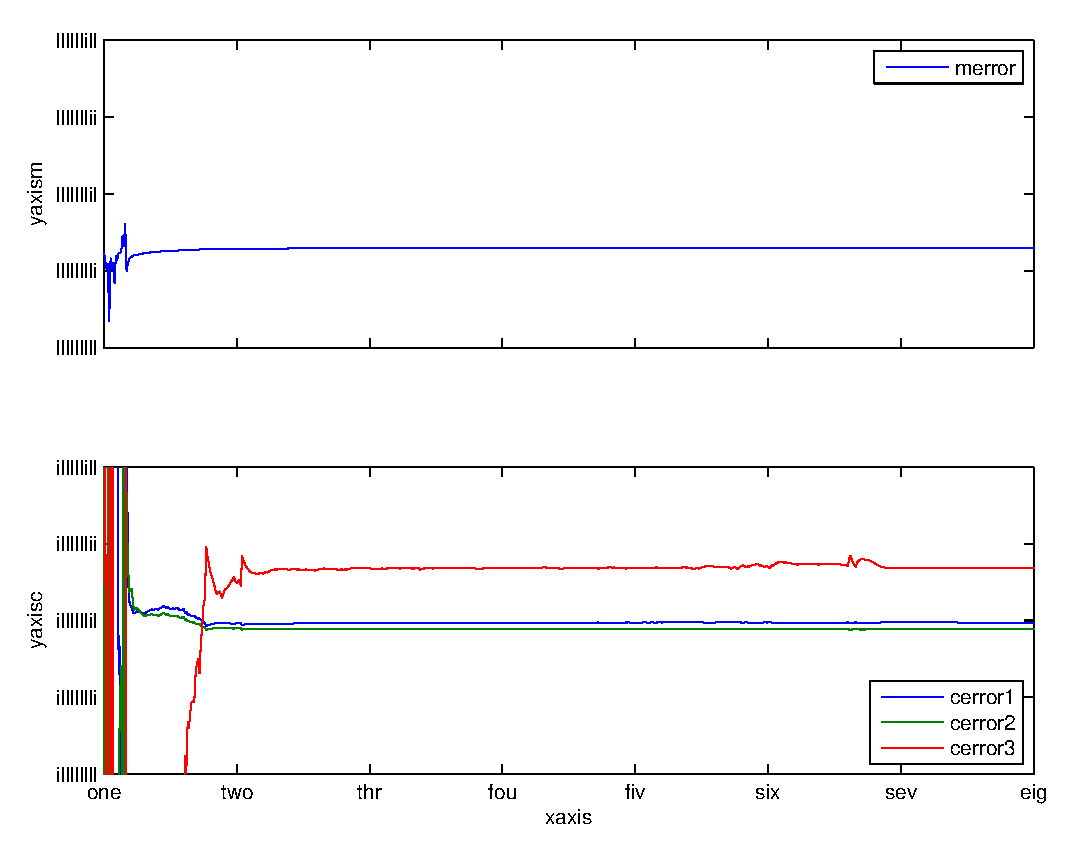
\includegraphics[width=0.8\textwidth]{figures/one_grasping_point_no_movement_mass_and_cog.eps}
	\vspace{0.2cm}
	\caption[Mass error, one grasping point, no excitation]{Mass $m$ and center of mass $\vec{c}$ errors with one grasping point and no excitation}
	\label{fig:estim_mass_one_no_movement}
\end{figure}

\begin{figure}
	\centering	
	\psfrag{xaxis}[tr][br]{$t\left[\mathrm{s}\right]$}
	\psfrag{yaxis}[bc][tr]{$\epsilon_\scr{I}\left[\scr{kg}/\scr{m}^2\right]$}
	\psfrag{one}[c][Br]{$0$}
	\psfrag{two}[c][Br]{$1$}
	\psfrag{thr}[c][Br]{$2$}
	\psfrag{fou}[c][Br]{$3$}
	\psfrag{fiv}[c][Br]{$4$}
	\psfrag{six}[c][Br]{$5$}
	\psfrag{sev}[c][Br]{$6$}
	\psfrag{eig}[c][Br]{$7$}
	\psfrag{lllllllll}[Br][Bl]{$-0.1\  $}
	\psfrag{lllllllli}[Br][Bl]{$-0.05\ $}
	\psfrag{lllllllil}[Br][Bl]{$0\  $}
	\psfrag{lllllllii}[Br][Bl]{$0.05\  $}
	\psfrag{llllllill}[Br][Bl]{$0.1\  $}
	\psfrag{Ixxerror}[][]{\tiny \hspace{0.5cm} $I_{xx,\scr{err}}$}
	\psfrag{Iyyerror}[][]{\tiny \hspace{0.5cm} $I_{yy,\scr{err}}$}
	\psfrag{Izzerror}[][]{\tiny \hspace{0.5cm} $I_{zz,\scr{err}}$}
	\psfrag{Ixyerror}[][]{\tiny \hspace{0.5cm} $I_{xy,\scr{err}}$}
	\psfrag{Ixzerror}[][]{\tiny \hspace{0.5cm} $I_{xz,\scr{err}}$}
	\psfrag{Iyzerror}[][]{\tiny \hspace{0.5cm} $I_{yz,\scr{err}}$}
	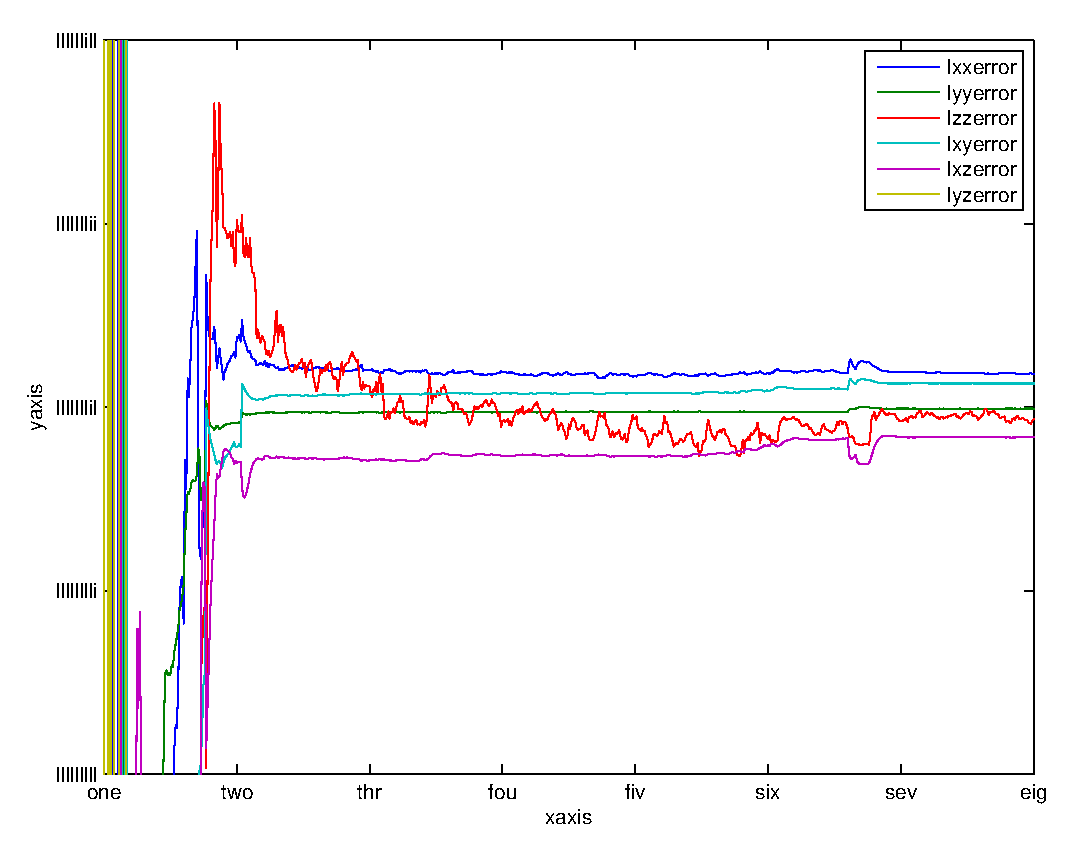
\includegraphics[width=0.8\textwidth]{figures/one_grasping_point_no_movement_inertias.eps}
	\vspace{0.2cm}
	\caption[Inertia errors, one grasping point, no excitation]{Inertia Tensor $\vec{I}_\scr{p}$ errors with one grasping point and no excitation}
	\label{fig:estim_inertia_one_no_movement}
\end{figure}

\begin{figure}
	\centering	
	\psfrag{xaxis}[tr][br]{$t\left[\mathrm{s}\right]$}
	\psfrag{yaxism}[bc][tr]{$\epsilon_\scr{m}\left[\mathrm{kg}\right]$}
	\psfrag{yaxisc}[bc][tr]{$\epsilon_\scr{CoM}\left[\mathrm{m}\right]$}
	\psfrag{one}[c][Br]{$0$}
	\psfrag{two}[c][Br]{$1$}
	\psfrag{thr}[c][Br]{$2$}
	\psfrag{fou}[c][Br]{$3$}
	\psfrag{fiv}[c][Br]{$4$}
	\psfrag{six}[c][Br]{$5$}
	\psfrag{sev}[c][Br]{$6$}
	\psfrag{eig}[c][Br]{$7$}
	\psfrag{lllllllll}[Br][Bl]{$-0.1\  $}
	\psfrag{lllllllli}[Br][Bl]{$0\ $}
	\psfrag{lllllllil}[Br][Bl]{$0.1\  $}
	\psfrag{illllllll}[Br][Bl]{$-0.1\  $}
	\psfrag{illllllli}[Br][Bl]{$-0.05\ $}
	\psfrag{illllllil}[Br][Bl]{$0\  $}
	\psfrag{illllllii}[Br][Bl]{$0.05\  $}
	\psfrag{illlllill}[Br][Bl]{$0.1\  $}
	\psfrag{cerror1}[][]{\tiny $c_{x,\scr{err}}$}
	\psfrag{cerror2}[][]{\tiny $c_{y,\scr{err}}$}
	\psfrag{cerror3}[][]{\tiny $c_{z,\scr{err}}$}
	\psfrag{merror}[][]{\tiny $m_{\scr{err}}$}
	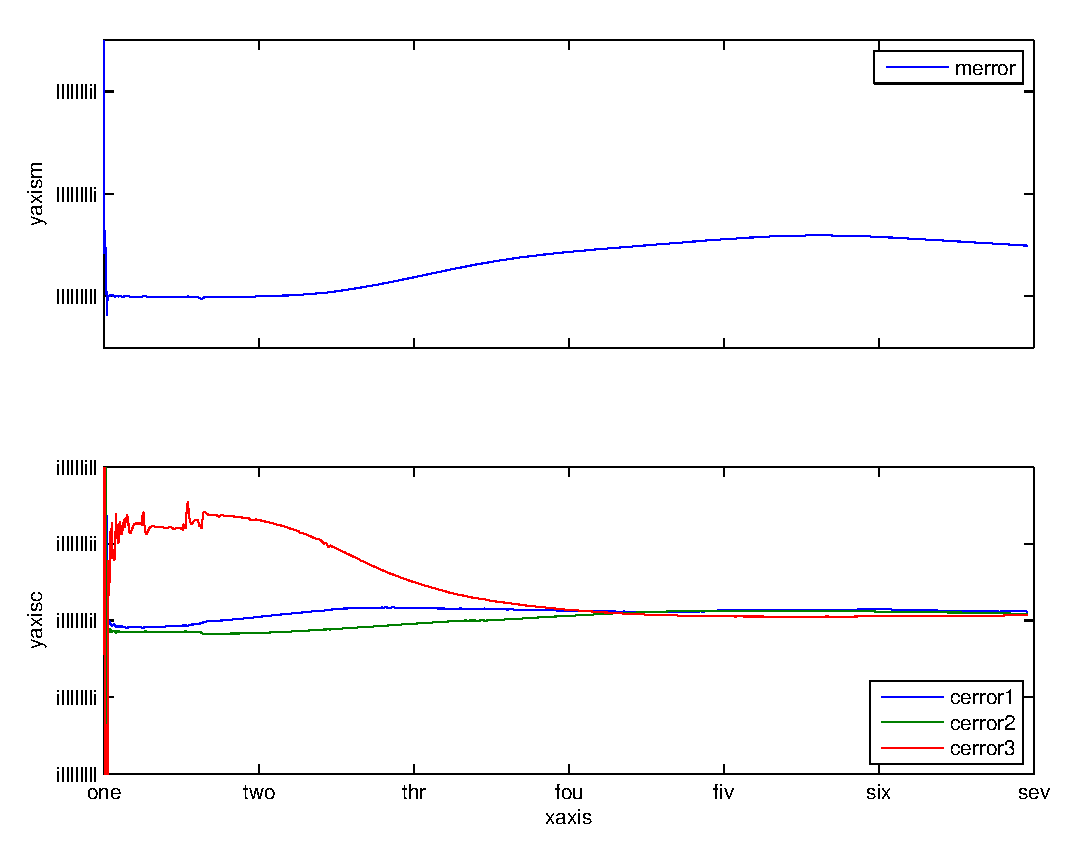
\includegraphics[width=0.8\textwidth]{figures/one_grasping_point_slow_mass_and_cog.eps}
	\vspace{0.2cm}
	\caption[Mass error, one grasping point, slow excitation]{Mass $m$ and center of mass $\vec{c}$ errors with one grasping point and slow excitation}
	\label{fig:estim_mass_one_slow}
\end{figure}

\begin{figure}
	\centering	
	\psfrag{xaxis}[tr][br]{$t\left[\mathrm{s}\right]$}
	\psfrag{yaxis}[bc][tr]{$\epsilon_\scr{I}\left[\scr{kg}/\scr{m}^2\right]$}
	\psfrag{one}[c][Br]{$0$}
	\psfrag{two}[c][Br]{$1$}
	\psfrag{thr}[c][Br]{$2$}
	\psfrag{fou}[c][Br]{$3$}
	\psfrag{fiv}[c][Br]{$4$}
	\psfrag{six}[c][Br]{$5$}
	\psfrag{sev}[c][Br]{$6$}
	\psfrag{eig}[c][Br]{$7$}
	\psfrag{lllllllll}[Br][Bl]{$-0.01\  $}
	\psfrag{lllllllli}[Br][Bl]{$-0.005\ $}
	\psfrag{lllllllil}[Br][Bl]{$0\  $}
	\psfrag{lllllllii}[Br][Bl]{$0.005\  $}
	\psfrag{llllllill}[Br][Bl]{$0.01\  $}
	\psfrag{Ixxerror}[][]{\tiny \hspace{0.5cm} $I_{xx,\scr{err}}$}
	\psfrag{Iyyerror}[][]{\tiny \hspace{0.5cm} $I_{yy,\scr{err}}$}
	\psfrag{Izzerror}[][]{\tiny \hspace{0.5cm} $I_{zz,\scr{err}}$}
	\psfrag{Ixyerror}[][]{\tiny \hspace{0.5cm} $I_{xy,\scr{err}}$}
	\psfrag{Ixzerror}[][]{\tiny \hspace{0.5cm} $I_{xz,\scr{err}}$}
	\psfrag{Iyzerror}[][]{\tiny \hspace{0.5cm} $I_{yz,\scr{err}}$}
	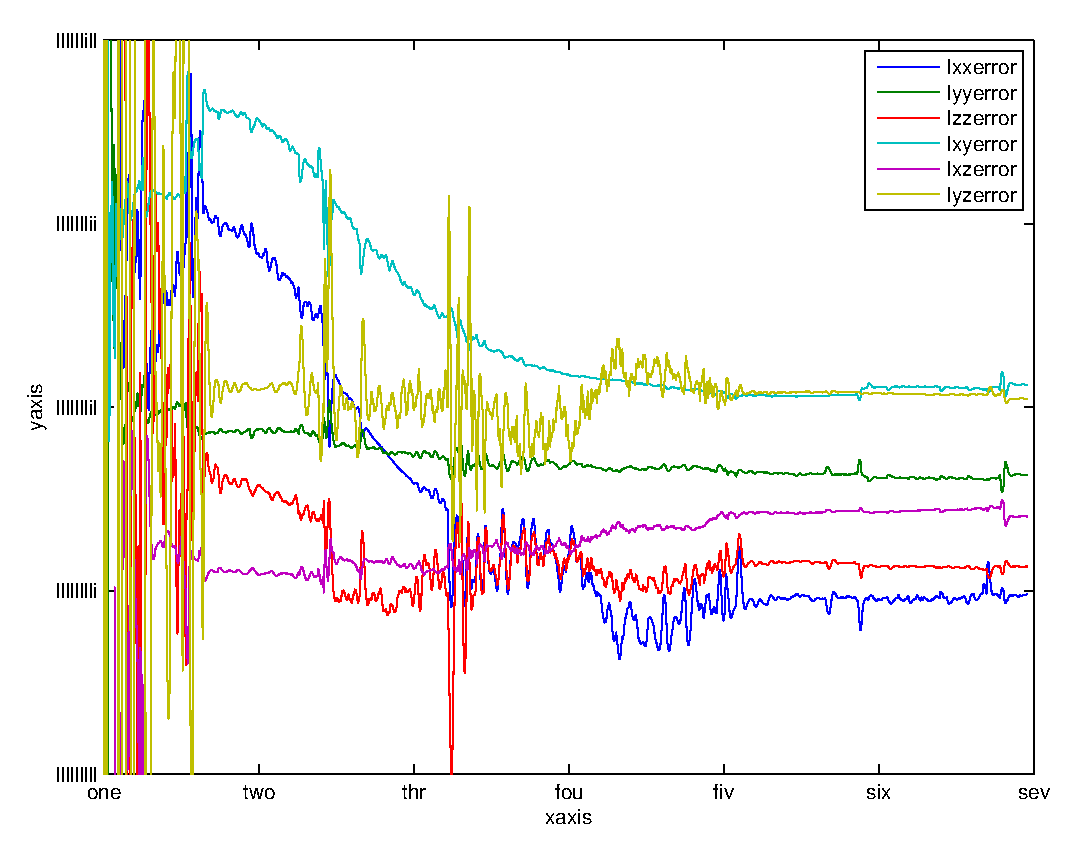
\includegraphics[width=0.8\textwidth]{figures/one_grasping_point_slow_inertias.eps}
	\vspace{0.2cm}
	\caption[Inertia errors, one grasping point, slow excitation]{Inertia Tensor $\vec{I}_\scr{p}$ errors with one grasping point and slow excitation}
	\label{fig:estim_inertia_one_slow}
\end{figure}

\begin{figure}
	\centering	
	\psfrag{xaxis}[tr][br]{$t\left[\mathrm{s}\right]$}
	\psfrag{yaxism}[bc][tr]{$\epsilon_\scr{m}\left[\mathrm{kg}\right]$}
	\psfrag{yaxisc}[bc][tr]{$\epsilon_\scr{CoM}\left[\mathrm{m}\right]$}
	\psfrag{one}[c][Br]{$0$}
	\psfrag{two}[c][Br]{$1$}
	\psfrag{thr}[c][Br]{$2$}
	\psfrag{fou}[c][Br]{$3$}
	\psfrag{fiv}[c][Br]{$4$}
	\psfrag{six}[c][Br]{$5$}
	\psfrag{sev}[c][Br]{$6$}
	\psfrag{eig}[c][Br]{$7$}
	\psfrag{lllllllll}[Br][Bl]{$-0.3\  $}
	\psfrag{lllllllli}[Br][Bl]{$-0.15\ $}
	\psfrag{lllllllil}[Br][Bl]{$0\  $}
	\psfrag{lllllllii}[Br][Bl]{$0.15\  $}
	\psfrag{llllllill}[Br][Bl]{$0.3\  $}
	\psfrag{illllllll}[Br][Bl]{$-0.2\  $}
	\psfrag{illllllli}[Br][Bl]{$-0.1\ $}
	\psfrag{illllllil}[Br][Bl]{$0\  $}
	\psfrag{illllllii}[Br][Bl]{$0.1\  $}
	\psfrag{illlllill}[Br][Bl]{$0.2\  $}
	\psfrag{cerror1}[][]{\tiny $c_{x,\scr{err}}$}
	\psfrag{cerror2}[][]{\tiny $c_{y,\scr{err}}$}
	\psfrag{cerror3}[][]{\tiny $c_{z,\scr{err}}$}
	\psfrag{merror}[][]{\tiny $m_{\scr{err}}$}
	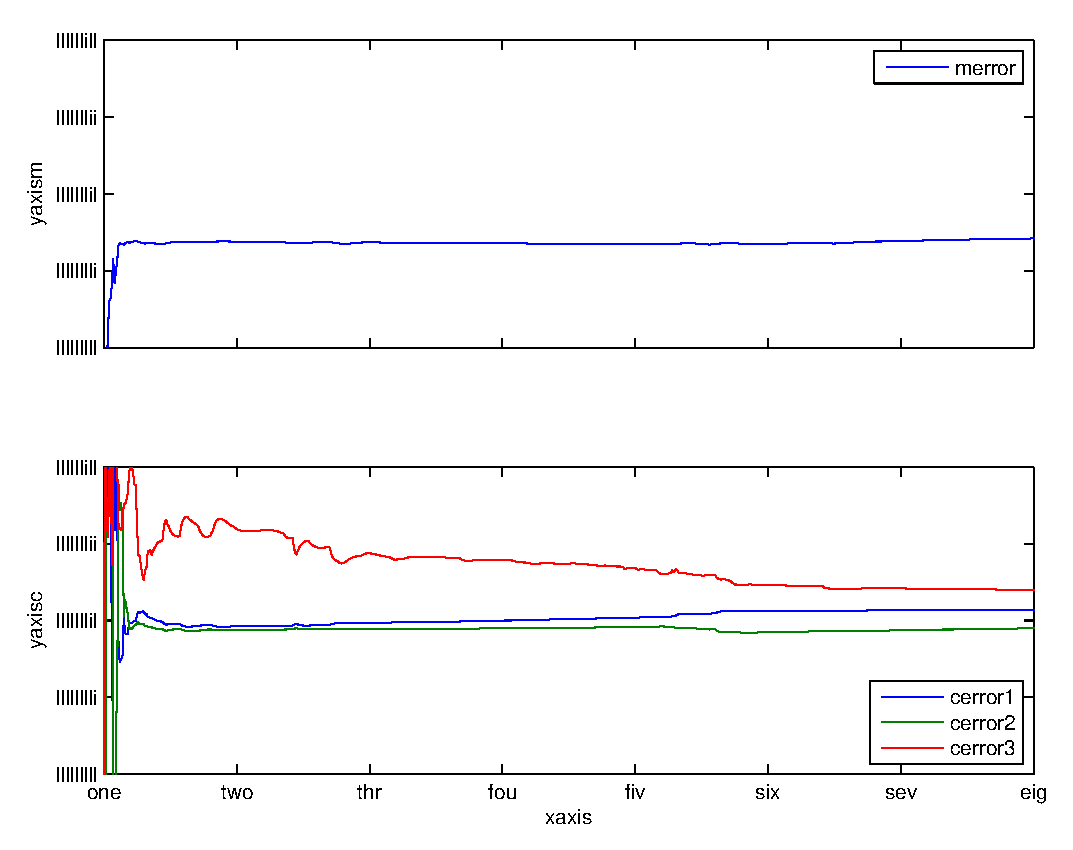
\includegraphics[width=0.8\textwidth]{figures/one_grasping_point_fast_mass_and_cog.eps}
	\vspace{0.2cm}
	\caption[Mass error, one grasping point, fast excitation]{Mass $m$ and center of mass $\vec{c}$ errors with one grasping point and fast excitation}
	\label{fig:estim_mass_one_fast}
\end{figure}

\begin{figure}
	\centering	
	\psfrag{xaxis}[tr][br]{$t\left[\mathrm{s}\right]$}
	\psfrag{yaxis}[bc][tr]{$\epsilon_\scr{I}\left[\scr{kg}/\scr{m}^2\right]$}
	\psfrag{one}[c][Br]{$0$}
	\psfrag{two}[c][Br]{$1$}
	\psfrag{thr}[c][Br]{$2$}
	\psfrag{fou}[c][Br]{$3$}
	\psfrag{fiv}[c][Br]{$4$}
	\psfrag{six}[c][Br]{$5$}
	\psfrag{sev}[c][Br]{$6$}
	\psfrag{eig}[c][Br]{$7$}
	\psfrag{lllllllll}[Br][Bl]{$-0.02\  $}
	\psfrag{lllllllli}[Br][Bl]{$-0.01\ $}
	\psfrag{lllllllil}[Br][Bl]{$0\  $}
	\psfrag{lllllllii}[Br][Bl]{$0.01\  $}
	\psfrag{llllllill}[Br][Bl]{$0.02\  $}
	\psfrag{Ixxerror}[][]{\tiny \hspace{0.5cm} $I_{xx,\scr{err}}$}
	\psfrag{Iyyerror}[][]{\tiny \hspace{0.5cm} $I_{yy,\scr{err}}$}
	\psfrag{Izzerror}[][]{\tiny \hspace{0.5cm} $I_{zz,\scr{err}}$}
	\psfrag{Ixyerror}[][]{\tiny \hspace{0.5cm} $I_{xy,\scr{err}}$}
	\psfrag{Ixzerror}[][]{\tiny \hspace{0.5cm} $I_{xz,\scr{err}}$}
	\psfrag{Iyzerror}[][]{\tiny \hspace{0.5cm} $I_{yz,\scr{err}}$}
	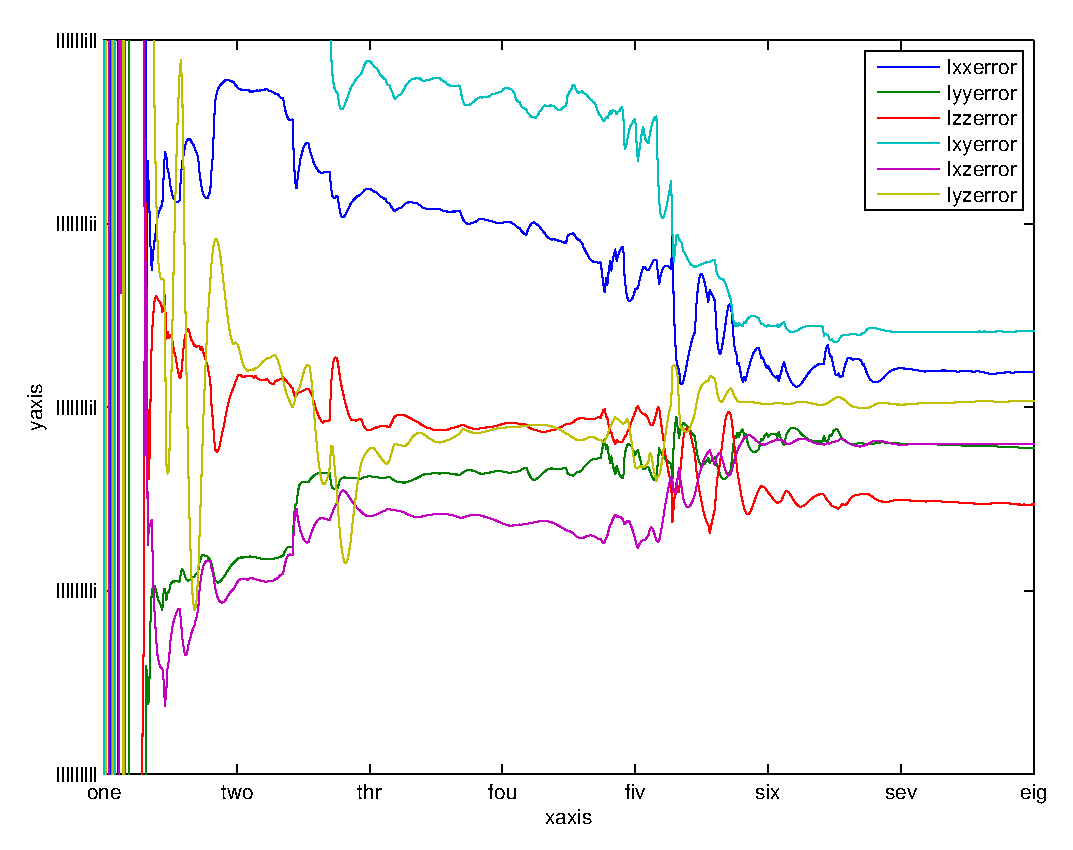
\includegraphics[width=0.8\textwidth]{figures/one_grasping_point_fast_inertias.eps}
	\vspace{0.2cm}
	\caption[Inertia errors, one grasping point, fast excitation]{Inertia Tensor $\vec{I}_\scr{p}$ errors with one grasping point and fast excitation}
	\label{fig:estim_inertia_one_fast}
\end{figure}

\subsection{Load Identification: Human-Robot Cooperation}

\chapter{Conclusion \& Outlook}

$\left(...\right)$ Conclusion $\left(...\right)$


As mentioned before, there exists a strong dependency between the choice of actuation pattern and the correct convergence of the estimation. Furthermore, we were able to design perturbation trajectories that significantly improve the convergence of one specific unknown parameter. The component $c_\scr{z}$ does not converge to the correct value unless the actuation pattern contains major rotations around the x-axis or the y-axis, just to name an example. Due to limitations on both the human and the robotic side it is however not possible to simply superpose the perturbation patterns to a pattern that leads to the convergence of all parameters at once. Thus, one possible improvement of the current estimation scheme could be a sequential parameter estimation. In a fist movement sequence, the object mass $m$ is estimated. Having estimated the mass, one proceeds to the again component-wise estimation of the center of mass $\vec{c}$. Again, having estimated the center of mass, one proceeds to apply a distinct pattern which allows a component-wise estimation of the object inertia $\vec{I}$.

Another advantageous adaptation to the presented data acquisition scheme could be the incorporation of inertial measurement units (IMUs). Firstly, the location of estimation experiment wouldn't be bound to a motion capture system. Secondly, the current motion-tracker cannot export quaternions and is thus affected by undesired singularities. Of course one has to take into account that the currently available IMU sensors are not able to provide sub-millimetre precision.


The overall estimation procedure is mainly bound by the robot actuator limits. The robot can not follow trajectories that include complex or fast motions (rotation 3-DoF, translation 3-DoF + rotation). These complex motions are required in order to achieve a convergence of all parameters. The estimation procedure could however be adapted to a human-human estimation with only little effort.
